\documentclass[12pt,a4paper,final,leqno]{report}
\usepackage[utf8]{inputenc}
\usepackage[norsk]{babel}
\usepackage{amsmath}
\usepackage{amsfonts}
\usepackage{amssymb}
\usepackage{graphicx}
\usepackage{float}
\usepackage[left=2cm,right=2cm,top=2cm,bottom=2cm]{geometry}
\usepackage{color}
\usepackage{pdfpages}
\sloppy
\definecolor{lightgray}{gray}{0.5}
\setlength{\parindent}{0pt}
\author{Krister Borge }
\title{FYS1120 Oblig2}
\makeindex
\begin{document}
\maketitle

%\newpage

%\newpage
\chapter*{Oppgave 1 test}
\section*{Oppgave 1: Partikkel i elektrisk felt: Programkode og verifisering}
I denne oppgaven har jeg brukt matlab til å plotte numerisk ved hjelp av Euler-Cromers metode for å fine hastihet og posisjon til en partikkel i et elektrisk felt. Det elektriske feltet \textbf{E}$=(-5$NC$^{-1},0,0)$ og initialverdiene r(t$=0$)$=(0,0,0)$ og v(t$=0$)$=(0,0,0)$. 
Jeg ser på intervallet $t_0=0$ til $t_1=1 \mu s$ 

$\Delta t=1n s $ og $\Delta t= 100n s$

\begin{verbatim}
function [  ] = oblig2oppgave1( dt )

E = [-5,0,0]; 
r0 = [0,0,0]; 
v0 = [0,0,0]; 
m_e = 9.11e-31; 
e = -1.6e-19; 

t0 = 0; 
t1 = 1*10e-6; 
% F og aksellerasjon 
F = e.*E; 
a = F./m_e; 
% initalverdier
r = r0;
v = v0; 
%t = linspace(t0,t1,(t1/dt)+1); 
ra = r0;
% Euler-Cromer method 
n = t1/dt
 t=0;
 c=0;
for i=2:n 
    v(i,:) = v(i-1,:) + a.*dt; 
    r(i,:) = r(i-1,:) + v(i,:).*dt; 
    c=c+dt;
    t(i,:)=c;
    %analytic
    ra(i,:) = 0.5.*(a.*c^2);
end 


%plotene 
%%

plot(t(:,1),r(:,1),'g',t(:,1), ra(:,1), 'r') 
axis('auto');
legend('Numerisk løsning', 'analytisk løsning'); title(['Oppgave 1 dt=', num2str(dt), 'ps']) 
xlabel('t'); ylabel('r') 
% hver komponent:
 %%
E=[-1, -2, 5];
F = e.*E; 
a = F./m_e; 
% initalverdier
r = r0;
v = v0; 
%t = linspace(t0,t1,(t1/dt)+1); 
ra = r0;
% Euler-Cromer method 
n = t1/dt; 
t=0;
c=0;
 for i=2:n 
    v(i,:) = v(i-1,:) + a.*dt; 
    r(i,:) = r(i-1,:) + v(i,:).*dt; 
    c=c+dt;
    t(i,:)=c;
 end

%plot
figure()
plot(t(:,1),r(:,1),'g', t(:,1), r(:,2), 'r', t(:,1), r(:,3), 'b')
legend('x_t', 'y_t', 'z_t')
xlabel('t'); ylabel('r') 
title('hver komponent tid posisjon')
figure()
plot3(r(:,1), r(:,2),r(:,3))
title('path'); grid();
xlabel('x_t'); ylabel('y_t'); zlabel('z_t')



end

\end{verbatim}

\begin{figure}[H]
\caption{Analytisk og numerisk løsning $\Delta t=1ns$}
\centering
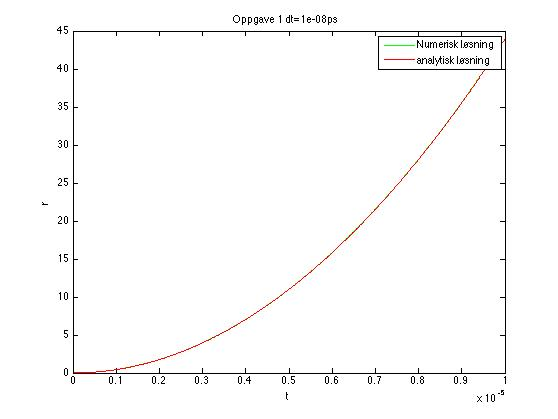
\includegraphics[width=\textwidth]{oppgave1analyticnumeric.jpg}
\end{figure}
\begin{figure}[H]
\caption{Analytisk og numerisk løsning $\Delta t=100ns$}
\centering
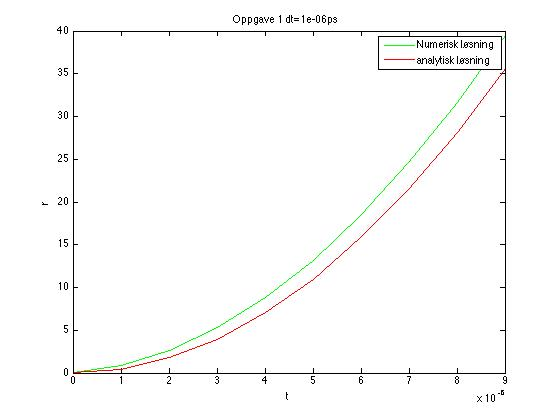
\includegraphics[width=\textwidth]{oppgave1analyticnumericdt2.jpg}
\end{figure}
\begin{figure}[H]
\caption{r$_x$ r$_y$ og r$_z$}
\centering
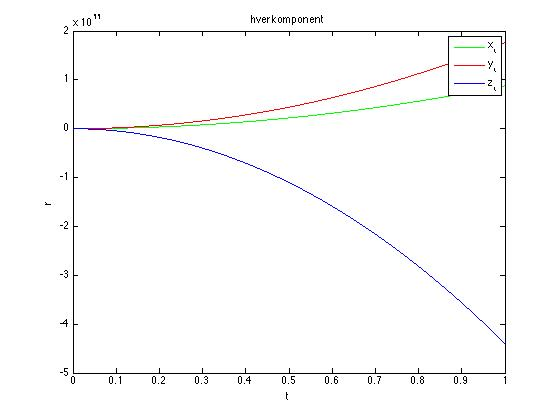
\includegraphics[width=\textwidth]{oppgave1component.jpg}
\end{figure}
\begin{figure}[H]
\caption{Banen i 3d}
\centering
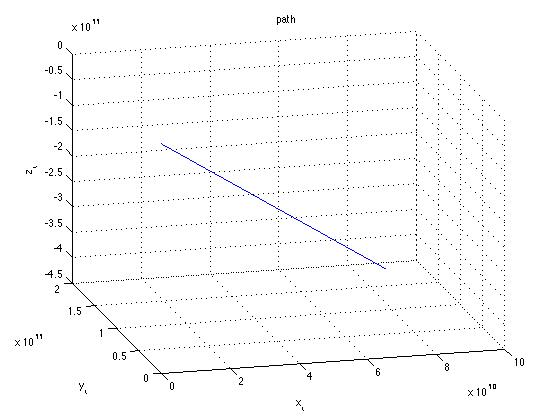
\includegraphics[width=\textwidth]{oppgave1path3d.jpg}
\end{figure}



\newpage
\chapter*{Oppgave 2}
\section*{Oppgave 2: Partikkel i magnetisk felt}
I denne oppgaven bruker jeg de den samme partikkelen som i oppgave 1. Euler-Cromers metode for å finne posisjon og fart.
\begin{verbatim}
%oppgave 2:
m_e = 9.11e-31; 
e = -1.6e-19; 
r0=[0 0 0];
v0=[10 0 0];
B=[0 0 5];
t0=0;
t1=1*10e-12;
dt=10e-15; %30fs
r=r0;
v=v0;
n=t1/dt;
t=t0;
c=0;

%F=e*(cross(v,B)

for i=2:n
    F = e*(cross(v(i-1,:),B));
    a = F./m_e; 
    v(i,:) = v(i-1,:) + a.*dt;
    r(i,:) = r(i-1,:) + v(i-1,:).*dt; 
    c=c+dt;
    t(i,:)=c;
end
oblig2oppgave2b(r,dt);
figure() 
plot(t(:,1),r(:,1),t(:,1),r(:,2),t(:,1),r(:,3))  
legend('r_x(t)','r_y(t)','r_z(t)'); title('Oppgave 2a tid posisjon') 
xlabel('tid'); ylabel('posisjon') 

figure() 
plot(t(:,1),v(:,1),t(:,1),v(:,2),t(:,1),v(:,3)) 
legend('v_x(t)','v_y(t)','v_z(t)'); title('Oppgave 2a tid hastighet ') 
xlabel('tid'); ylabel('hastighet') 

figure() 
plot3(r(:,1),r(:,2),r(:,3)) 
legend('path'); title('Oppgave 2a Path i 3d'); grid() 
xlabel('r_x'); ylabel('r_y'); zlabel('r_z')

clear all

\end{verbatim}
\subsection*{Oppgave 2 a)}
\begin{figure}[H]
\caption{Posisjon}
\centering
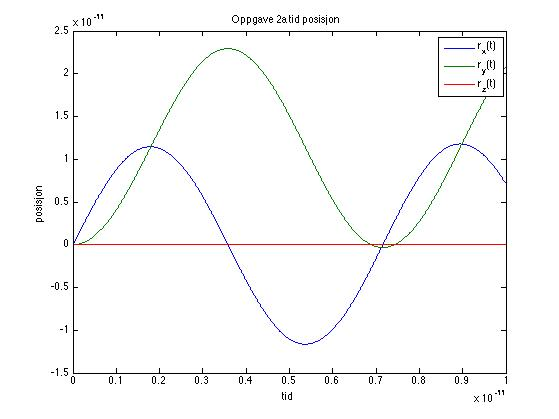
\includegraphics[width=\textwidth]{oppgave2rt.jpg}
\end{figure}
\begin{figure}[H]
\caption{Fart}
\centering
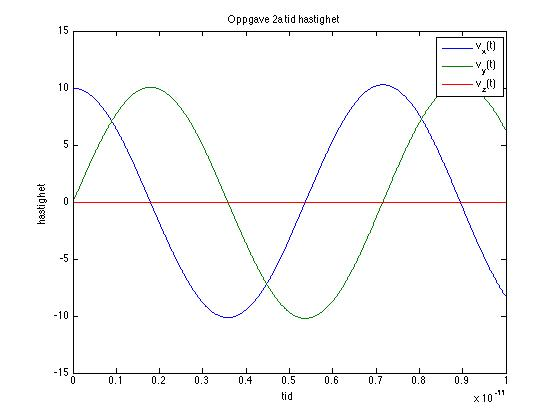
\includegraphics[width=\textwidth]{oppgave2vt.jpg}
\end{figure}
\begin{figure}[H]
\caption{3d}
\centering
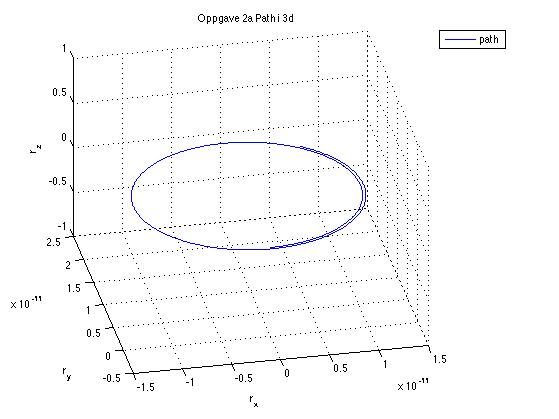
\includegraphics[width=\textwidth]{oppgave23d.jpg}
\end{figure}
\subsection*{Oppgave 2 b)}
Måler omløpstiden T:
\begin{verbatim}
function [  ] = oblig2oppgave2b( r, dt )
%oblig2oppgave2b 
%   oppgave 2b regner ut omløpstiden T:

T=0;
for j=1:n
    if (-dt< r(j,1)> dt)
        r(j);
        T=j;
    end    
end
T=T*2*dt;
format=('Omløpstiden %s \n');
fprintf(format,T)
% Omløpstiden 1.790000e-11 
end
\end{verbatim}
\subsection*{Oppgave 2 c)}
 Vis analytisk at syklotronfrekvensen til dette systemet er
 $$
 \omega_c=\frac{q\mathsf{B}}{m}
 $$
 der B=$|\mathbf{B}|$ bruker dette til å vise at
 $$
T=\frac{2\pi m}{q\mathsf{B}}
$$

Jeg vet at F$=ma$ og at v$=\frac{d}{t}$
Skriver F$=m\frac{v^2}{r}$ slik at $qvB=\frac{mv^2}{r}$ og løser for $r$.
$$
qB=\frac{mv}{r}r=>\frac{mv}{qB}
$$
Jeg ser videre på $v=\frac{d}{t}=\frac{2\pi r}{T}$ som gir $T=\frac{2\pi r}{v}$
Setter inn for $r=\frac{mv}{qB} $ og får:
$$
T=\frac{2\pi m}{qB}
$$

\subsection*{Oppgave 2 d)}
\begin{verbatim}
%oppgave 2d


m_e = 9.11e-31; 
e = -1.6e-19; 
r0=[0 0 0];

v0=[5 0 2];

B=[0 0 5];
t0=0;
t1=1*10e-12;
dt=10e-15; %30fs
r=r0;
v=v0;
n=t1/dt;
t=t0;
c=0;
for i=2:n
    F = e*(cross(v(i-1,:),B));
    a = F./m_e; 
    v(i,:) = v(i-1,:) + a.*dt;
    r(i,:) = r(i-1,:) + v(i-1,:).*dt; 
    c=c+dt;
    t(i,:)=c;
end
figure() 
plot(t(:,1),v(:,1),t(:,1),v(:,2),t(:,1),v(:,3)) 
legend('v_x(t)','v_y(t)','v_z(t)'); title('Oppgave 2d tid hastighet ') 
xlabel('tid'); ylabel('hastighet') 

figure() 
plot3(r(:,1),r(:,2),r(:,3)) 
legend('path'); title('Oppgave 2d Path i 3d'); grid() 
xlabel('r_x'); ylabel('r_y'); zlabel('r_z')
\end{verbatim}

\begin{figure}[H]
\caption{Oppgave 2d - Fart}
\centering
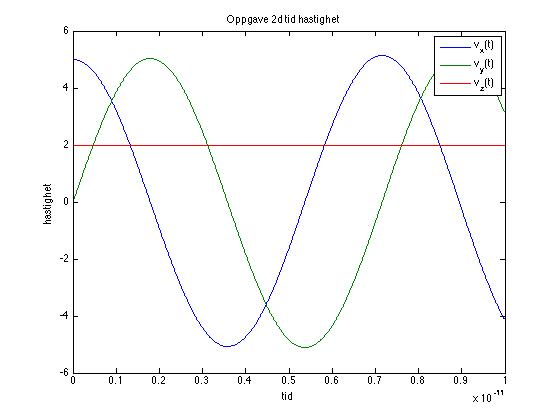
\includegraphics[width=\textwidth]{oppgave2dvt.jpg}
\end{figure}

\begin{figure}[H]
\caption{Oppgave 2 d - 3d}
\centering
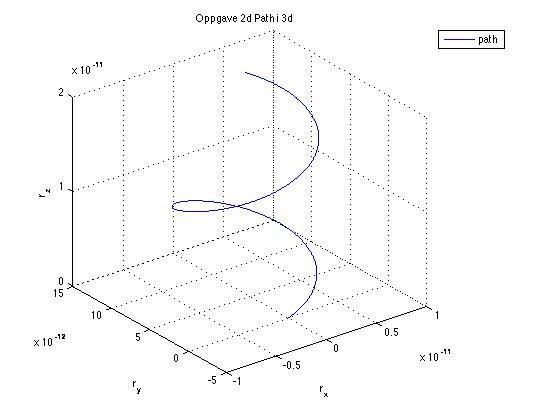
\includegraphics[width=\textwidth]{oppgave2d3d.jpg}
\end{figure}



\chapter*{Oppgave 3 - Partikkel i syklotron}
\subsection*{Oppgave 3 a}
I denne oppgaven ser vi på en partikkels bane i magnetfelt og elektrisk felt.

$$E = \begin{cases} E_0cos(\omega t) \hat{\mathbf{e}}_x, & \mbox{hvis } x \in (d/2, -d/2) \\ (0, 0, 0) & \mbox{ellers}\end{cases}$$

Systemet ser på banen partikllen i feltet.
 
\begin{verbatim}
% variabler
m_p = 1.67*10e-27;
e = 1.6*10e-19;
v0 = [0,0,0];
r0 = [0,0,0];
B = [0,0,2]; %B=(0,0,2T)
dt = 1e-10;
t0 = 0;
t1 = 3e-6;
t=t0:dt:t1;
r = r0;
v = v0;
E0 = [90/25 0 0 ];
E=E0;
Bs=sqrt(B(:,1)^2 + B(:,2)^2 +B(:,3)^2) ; 
omega = (e*Bs)/m_p;
for i=2:length(t)
    
    F_B = e.*(cross(v(i-1,:),B));
    F_E = E.*e;
    F = F_E+F_B;
    a = F./m_p;
    v(i,:) = v(i-1,:) + a.*dt;
    r(i,:) = r(i-1,:) + v(i-1,:).*dt;
    if (r(i-1,1) <= 0.1 && r(i-1,1) >= -0.1)
        E = E0.*cos(omega*t(i).*[1 0 0]);
        
    else
        E = [0,0,0];
    end
end
figure()
plot(r(:,1), r(:,2))
legend('bane'); title('Oppgave 3a')
xlabel('x_t'); ylabel('y_t')

\end{verbatim}
\begin{figure}[H]
\caption{Oppgave 3a -$x_t$ mot $y_t$}
\centering
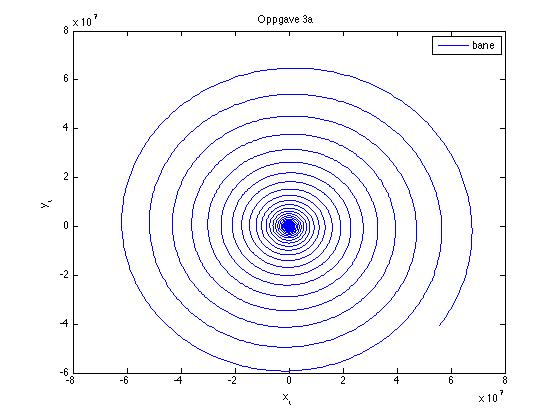
\includegraphics[width=\textwidth]{oppgave3a.jpg}
\end{figure}

Avstanden øker med hver runde. (FINN UT HVORFOR OG SKRIV HER!!)
\subsection*{Oppgave 3 b}
\begin{verbatim}

m_p = 1.67*10e-27;
e = 1.6*10e-19;
v0 = [0,0,0];
r0 = [0,0,0];
B = [0,0,2]; %B=(0,0,2T)
dt = 100e-12;
t0 = 0;
t1 = 300e-9;
t=t0:dt:t1;
r = r0;
v = v0;
E0 = [90/25 0 0 ];
E=E0;
Bs=sqrt(B(:,1)^2 + B(:,2)^2 +B(:,3)^2); 
omega = (e*Bs)/m_p;
r_d = 5e-2;
for i=2:length(t)
    
    F_B = e.*(cross(v(i-1,:),B));
    F_E = E.*e;
    F = F_E+F_B;
    a = F./m_p;
    v(i,:) = v(i-1,:) + a.*dt;
    r(i,:) = r(i-1,:) + v(i-1,:).*dt;
    if (r(i-1,1) <= r_d && r(i-1,1) >= -r_d)
        E = E0.*cos(omega*t(i).*[1 0 0]);
    else
        E = [0,0,0];
    end
end
figure()
plot(t,r(:,1), t,r(:,2), t, r(:, 3))
legend('x_t','y_t','z_t')
title('Oppgave 3b - position')
xlabel('time s'); ylabel('position')
figure()
plot(t,v(:,1), t,v(:,2), t, v(:, 3))
legend('v_x','v_y','v_z' )
title('Oppgave 3b - velocity')
xlabel('time s'); ylabel('velocity')

\end{verbatim}
\begin{figure}[H]
\caption{Posisjon}
\centering
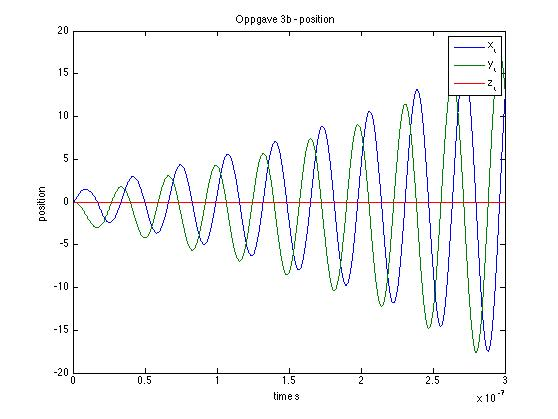
\includegraphics[width=\textwidth]{oppgave3br.jpg}
\end{figure}

\begin{figure}[H]
\caption{fart}
\centering
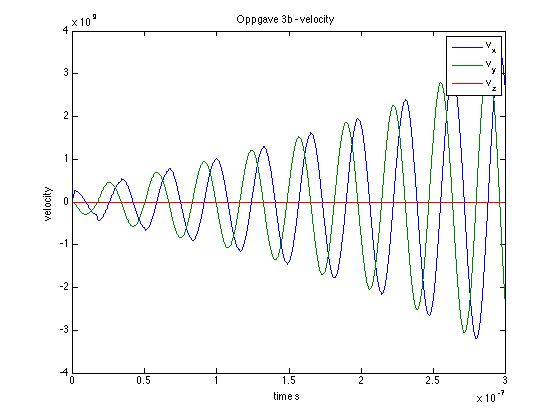
\includegraphics[width=\textwidth]{oppgave3bv.jpg}
\end{figure}
\subsection*{Oppgave 3 c)}
utvider programmet med
\begin{verbatim}
fart=sqrt(v(length(v)-1,1)^2+ v(length(v)-1,2)^2+v(length(v)-1,3)^2)
\end{verbatim}
Farten er da: 69.4221
\newpage
\subsection*{Oppgave 3 d)}
Jeg kan vise at den kinetiske enerigen er
$$
E_k=\frac{1}{2}\frac{q^2B^2r^2}{m}
$$
Jeg har at $E_k=\frac{1}{2} mv^2$  jeg vet videre at $v=\frac{qBr}{m}$  og at $r=\frac{mv}{qB}$ 

Setter inn :
$$
E_k=\frac{1}{2} m (\frac{qBr}{m})^2=\frac{1}{2} \frac{q^2B^2r^2}{m}
$$

finner løsningen for $E_k$ i MeV med et bittelite matlabskript
\begin{verbatim}
m_p = 1.67*10e-27;
q = 1.6*10e-19;
r = 0.5;
B=2;
E_k=0.5*((q^2*B^2*r^2)/(m_p))
E_kmev=E_k*6241509341896.7
%E_k = 7.6647e-11 joule
%E_kmev = 478.3911 MeV
\end{verbatim}
Den kinetiske energien er $E_k = 7.6647*10^{-11}$ Joule $=478.3911$ MeV.

\chapter*{Oppgave 4 - RC-krets} 
\subsection*{Oppgave 4a)}
\begin{figure}[H]
\caption{ Oppgave aRC-Krets }
\centering
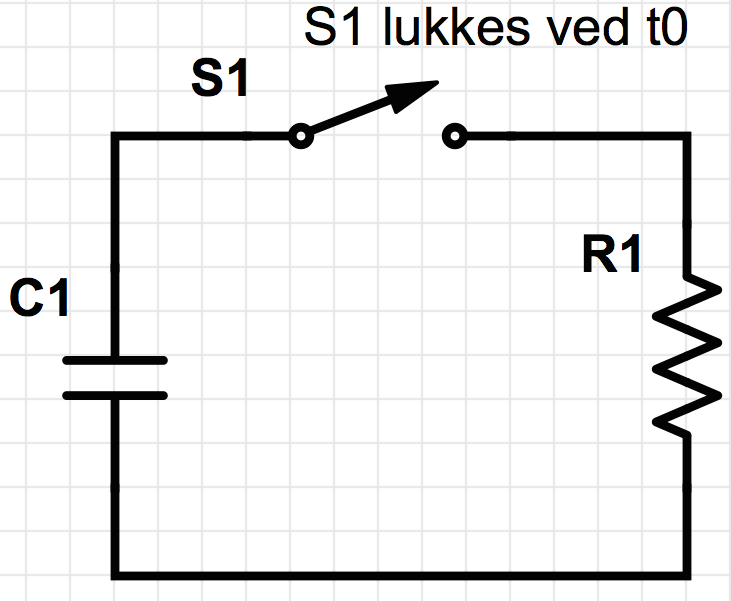
\includegraphics[width=\textwidth]{krets1.jpg}
\end{figure}
\subsection*{Oppgave 4b)}
Her er en krets med en bryter S1, en resistor R og en kondensator C. Ladningen på platene i C er $\pm Q$.

jeg kan finne strømmen i denne kretsen ved å bruke $C=\frac{Q}{V}$, Ohms lov $V=IR$ og definisjonen av strøm $I=\frac{dQ}{dt}$
$$
0=\frac{Q(t)}{C}+I(t)R
$$
$$
I(t)R=-\frac{Q(t)}{C} 
$$
Deler på R og får strømmen I
$$
I(t)=\frac{Q(t)}{RC}=\frac{Q(t)}{\tau}
$$
Definisjonen av strøm gir oss da:
$$
I(t)=\frac{dQ(t)}{dt}=\frac{Q(t)}{\tau}
$$
Ladningen på C faller derfor eksponensielt med tiden:
$$
Q(t)=Q_{max}e^{-\frac{t}{\tau}}
$$
\subsection*{Oppgave 4c}
Strømmen i kretsen er nådd halv parten av $I_max$ ved $0.69 \tau$ siden $e^-0.69\approx 0.5$

\subsection*{Oppgave 4c)}
Strømmen vil ha falt til halvparten av $Q_{max}$ etter 

\subsection*{Oppgave 4d)}
\begin{figure}[H]
\caption{RC-Krets med batteri med emf $\epsilon$}
\centering
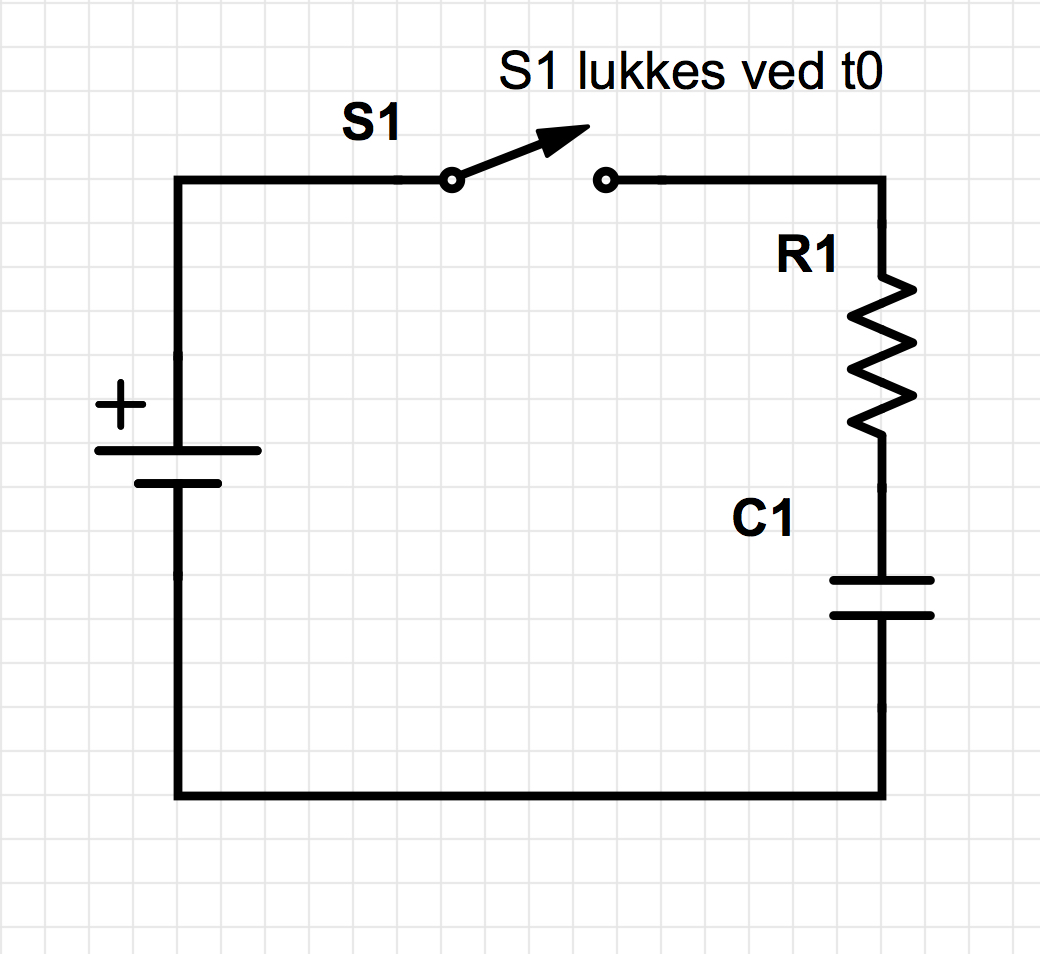
\includegraphics[width=\textwidth]{krets.jpg}
\end{figure}

Nå vil Kirchoff ha noe å si:
$$
\epsilon - V_C-V_R=0
$$
Skriver om 
$$\epsilon - \frac{Q}{C} -Ri=0
$$
$$
\epsilon- \frac{Q}{C}- R \frac{dq}{dt}=0
$$
$$
\frac{dq}{dt}=\frac{1}{RC}(Q-C\epsilon)
$$
$$
\frac{dq}{Q-C\epsilon }=-\frac{dt}{RC}
$$
Integrerer:
$$
\int \frac{dq}{Q-C\epsilon }=-\frac{1}{RC}\int dt
$$
Ladningen er gitt ved:
$$
Q=C\epsilon (1-e^{-t/\tau})
$$
Strømmen blir da:
$$
I=\frac{dQ}{dt}=\frac{\epsilon}{R} e^{-t/\tau}=I_0e^{-t/\tau}
$$
\chapter*{MatLab}
\includepdfmerge{oblig2oppgave1.pdf}
\includepdfmerge{oblig2oppgave2.pdf}
\includepdfmerge{oblig2oppgave2b.pdf}
\includepdfmerge{oblig2oppgave2d.pdf}
\includepdfmerge{oblig2oppgave3a.pdf}
\includepdfmerge{oblig2oppgave3b.pdf}
\includepdfmerge{oblig2oppgave3d.pdf}

\end{document}

